\selectlanguage{english}%

\chapter{Modelagem}

\section{Modelagem Convencional} \label{secModConvencional}
\subsection{Modelo Não Linear}
Baseado nos princípios de conservação de massa e na lei de Bernoulli para líquidos incompressíveis tem-se o seguinte sistema de equações não lineares que descrevem o processo.

\begin{equation}
	\begin{cases}
		\dot{h_{1}} = \frac{1}{A_{1}}(a_{3}\sqrt{2gh_{3}} + \gamma_{1}k_{1}v_{1} - a_{1}\sqrt{2gh_{1}})\\
		
		\dot{h_{2}} = \frac{1}{A_{2}}(a_{4}\sqrt{2gh_{4}} + \gamma_{2}k_{2}v_{2} - a_{2}\sqrt{2gh_{2}})\\
		
		\dot{h_{3}} = \frac{1}{A_{3}}((1 - \gamma_{2})k_{2}v_{2} - a_{3}\sqrt{2gh_{3}})\\
		
		\dot{h_{4}} = \frac{1}{A_{4}}((1 - \gamma_{1})k_{1}v_{1} - a_{4}\sqrt{2gh_{4}})
	\end{cases}
\end{equation}
em que, $h_{i}$, $A_{i}$ e $a_{i}$ são o nível de água, a área da secção transversal e a área de secção transversal do orifício de saída do tanque i, $i=1,2,3,4$, respectivamente. A constante de fluxo e a tensão aplicada na bomba j são dadas respectivamente por $k_{j}$ e $v_{i}$, $j=1,2$. O parâmetro $\gamma_{1}$ é a razão entre os fluxos para os tanques 1 e 4, $\gamma_{2}$ é a razão entre os fluxos para os tanques 2 e 3 e g é a aceleração da gravidade. 

\subsection{Linearização}
Linearizando o sistema em torno dos ponto de operação $\overline{h}=(\overline{h_{1}},\overline{h_{2}},\overline{h_{3}},\overline{h_{4}})$ e $\overline{v}=(\overline{v_{1}},\overline{v_{2}})$, por expansão em série de Taylor, obtém-se a seguinte representação no espaço de estados:

\begin{multline}
	\begin{bmatrix}
		\dot{\Delta h_{1}} \\
		\dot{\Delta h_{2}} \\
		\dot{\Delta h_{3}} \\
		\dot{\Delta h_{4}} 
	\end{bmatrix}
	= 
	\begin{bmatrix}
		\frac{-a_{1}\sqrt{2g}}{2A_{1}\sqrt{h_{1}}} & 0 & \frac{a_{3}\sqrt{2g}}{2A_{1}\sqrt{h_{3}}} & 0 \\
		0 & \frac{-a_{2}\sqrt{2g}}{2A_{2}\sqrt{h_{2}}} & 0 & \frac{a_{4}\sqrt{2g}}{2A_{2}\sqrt{h_{4}}} \\
		0 & 0 & \frac{-a_{3}\sqrt{2g}}{2A_{3}\sqrt{h_{3}}} & 0 \\
		0 & 0 & 0 & \frac{-a_{4}\sqrt{2g}}{2A_{4}\sqrt{h_{4}}}
	\end{bmatrix}
	\begin{bmatrix}
		\Delta h_{1} \\
		\Delta h_{2} \\
		\Delta h_{3} \\
		\Delta h_{4} 
	\end{bmatrix}
	\\+
	\begin{bmatrix}
		\frac{\gamma_{1}k_{1}}{A_{1}} & 0 \\
		0 & \frac{\gamma_{2}k_{2}}{A_{2}} \\
		0 & \frac{(1-\gamma_{2}) k_{2}}{A_{3}} \\
		\frac{(1-\gamma_{1})k_{1}}{A_{4}} & 0
	\end{bmatrix}
	\begin{bmatrix}
		\Delta v_{1} \\
		\Delta v_{2}
	\end{bmatrix}
	\label{eq2}
\end{multline}
\begin{equation}
	\begin{bmatrix}
		y_{1} \\
		y_{2} \\
		y_{3} \\
		y_{4} 
	\end{bmatrix}
	= 
	I
	\begin{bmatrix}
		\Delta h_{1} \\
		\Delta h_{2} \\
		\Delta h_{3} \\
		\Delta h_{4} 
	\end{bmatrix}
	\label{eq3}
\end{equation}

em que $y_{i}$ são as saídas medidas do sistema, $\Delta h_{i}=h_{i} - \overline{h_{i}}$, $\Delta v_{i}=v_{i} - \overline{v_{i}}$, e $i=1,2,3,4$.

E por fim, a matriz função de transferência do sistema obtida é:
\begin{equation}
	G(s) = 
	\begin{bmatrix}
		\frac{T_{1}\gamma_{1}k_{1}}{A_{1}(1+sT_{1})} &  \frac{T_{1}(1-\gamma_{2})k_{2}}{A_{1}(1+sT_{3})(1+sT_{1})} \\
		\frac{T_{2}(1-\gamma_{1})k_{1}}{A_{2}(1+sT_{4})(1+sT_{2})} &  \frac{T_{2}\gamma_{2}k_{2}}{A_{2}(1+sT_{2})} \\
		0 &  \frac{T_{3}(1-\gamma_{2})k_{2}}{A_{3}(1+sT_{3})} \\
		\frac{T_{4}(1-\gamma_{1})k_{1}}{A_{4}(1+sT_{4})} &  0 
	\end{bmatrix} 
	\label{eq4}
\end{equation}

em que $G(s)=\frac{\Delta h(s)}{\Delta v(s)}$ e $T_{i}=\frac{2A_{i}\sqrt{h_{i}}}{a_{i}\sqrt{2g}}$, $i=1,2,3,4$.

\section{Modelagem Fuzzy Takagi-Sugeno} \label{secModFuzzy}
\indent A Teoria Fuzzy tem seu princípio cunhado por \cite{zadeh65}. Os trabalhos seguintes, como o \cite{takagi_sugeno} abordaram sua utilização para a modelagem de sistemas complexos por meio de aproximações, utilizando uma teoria de conjuntos diferente da convencional.

\subsection{Conjuntos Fuzzy}
\indent A teoria de conjuntos convencional utiliza lógica booleana para definir os valores lógicos das funções de pertinências dos conjuntos. Assim, dado $X$ o universo de discurso de um determinado conjunto $C$, um elemento genérico $x$ tem sua função de pertinência ao conjunto $C$ dado por:

\begin{align*}
	f_{C}(x)&:X \rightarrow \{0,1\} \quad \\
	f_{C}(x)&= 
	\begin{cases}
		1 \text{ se e somente se x} \in C \\
		0 \text{ se e somente se x} \notin C\\
	\end{cases}
\end{align*}

Existem, no entanto, situações em que a definição dos conjuntos de seus limites se tornam muito subjetivos. Nestas situações, a utilização da lógica difusa apresenta vantagens para a modelagem de sistemas. 

Considere-se como exemplo a temperatura de uma sala. Pode-se definir dois conjuntos de estados \{quente,frio\}. No entanto, torna-se um pouco confuso e arbitrário decidir em qual destes conjuntos um estado específico se encaixa. Utilizando funções de pertinências não binárias, observa-se o \textbf{quanto} determinada temperatura se encaixa em cada um dos conjuntos. Funções de pertinências fuzzy são definidas da forma:

\begin{align*}
	f_{C}(x)&:X \rightarrow [0,1]
\end{align*}

\subsection{Funções De Pertinência}
Existem várias normas e regras disponíveis para funções de pertinência. Este trabalho considera a norma triangular. Seguindo o exemplo dado, dada uma temperatura $x$ verifica-se o quão pertencente aos conjuntos \textit{quente} e \textit{fria} ela é utilizando a função do gráfico a seguir:

\begin{figure}[H]
	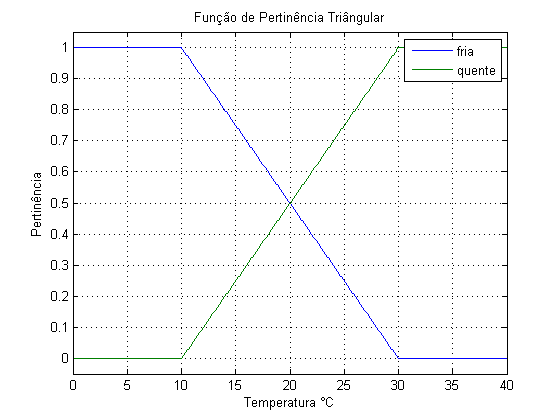
\includegraphics[width=0.5\textwidth]{img/pertinencia.png}
	\caption{Diagrama esquemático do sistema de quatro tanques e planta didática.}
	\label{figPertinencia}
\end{figure}

Nota-se que se escolhem limites para os conjuntos: toda temperatura abaixo de 10 é fria; toda temperatura acima de 30 é quente. As demais, pertencem mais ou menos à cada um dos conjuntos.

Em lógica Fuzzy, as variáveis definidas de forma subjetiva, com expressões para limites são chamadas variáveis linguísticas.

\subsection{Modelo Fuzzy Takagi-Sugeno}
A abordagem proposta por \cite{takagi_sugeno} promove a utilização da lógica fuzzy na modelagem e controle de sistemas. As etapas deste processo são:
\begin{itemize}
	
	\item \textbf{Fuzzificação:}
	Chamemos de $x_{i}$ e $C_{i}$, onde i=1,2,3...n, as n variáveis medidas de um sistema e os conjuntos fuzzy aos quais podem ou não pertencer, respectivamente. No modelo de Takagi-Sugeno temos as regras dadas da forma:
	SE $x_1$ é $A_1i$ e $x_1$ é $A_1i$ e $x_1$ é $A_1i$ e ... e $x_1$ é $A_1i$ ENTÂO $y = f_i(x_1, x_2, ..., X_n)$
	
	No objeto de estudos deste trabalho, as variáveis de entradas são os níveis $h_1$ e $h_2$. Para cada um deles pode se definir os conjuntos \{baixo, alto\} e modelar o sistema nas quatro combinações possíveis:
	\begin{itemize}
		\item Se $h_1$ é baixo e $h_2$ é baixo, então $\dot{x} = A_{1}x + B_{1}u$
		\item Se $h_1$ é baixo e $h_2$ é alto, então $\dot{x} = A_{2}x + B_{2}u$
		\item Se $h_1$ é alto e $h_2$ é baixo, então $\dot{x} = A_{3}x + B_{3}u$
		\item Se $h_1$ é alto e $h_2$ é alto, então $\dot{x} = A_{4}x + B_{4}u$
	\end{itemize}
	
	Com a regras já definidas, realiza-se o próximo passo para inferir o quanto o estado atual pertence a cada um dos estados e o sistema resultante.
	
	\item \textbf{Inferência:}
	As variáveis $h_1$ e $h_2$ são chamadas variáveis premissas. Obtém-se então o grau de compatibilidade dos níveis em cada um dos quatro conjuntos anteriores utilizando funções de pertinências triangulares, como apresentado anteriormente. Para este tipo de função, o peso final da regra é dado pelo produtório do grau de ativação das premissas em cada região. Ou seja, chamando de $w_i(h_1,h_2)$ este peso, temos:
	
	\begin{align*}
		w_1(h_1,h_2) &= f_{baixo}(h_1)*f_{baixo}(h_2) \\
		w_2(h_1,h_2) &= f_{baixo}(h_1)*f_{alto}(h_2) \\
		w_3(h_1,h_2) &= f_{alto}(h_1)*f_{baixo}(h_2) \\
		w_4(h_1,h_2) &= f_{alto}(h_1)*f_{alto}(h_2) \\
	\end{align*}
	
	Assim, o modelo Takagi-Sugeno final é dado por:
	\begin{align*}
		\dot{h} = \frac{\sum_{i=1}^{4}  w_i(h)(A_ih + B_i u)}{\sum_{i=1}^{4} w_i(h)}
	\end{align*}
	
	Nota-se que o número de regras é obtido a partir da combinação simples entre as variáveis de discurso. Além disso, é importante notar que se tratam de linearizações, portanto as variáveis utilizadas são todas desvios de cada um dos respectivos pontos de linearização, que portanto precisam ser previamente calculados e inseridos no modelo.
	
\end{itemize}

\selectlanguage{brazil}%

